 
%
\documentclass{llncs}
\usepackage{graphicx}      % include this line if your document contains figures
%\usepackage{natbib}        % required for bibliography
\usepackage{amsmath} 
\usepackage{amssymb}
\usepackage{tensor} 
\usepackage{cite}
\usepackage{graphicx}
\usepackage{floatrow}
% Table float box with bottom caption, box width adjusted to content
\newfloatcommand{capbtabbox}{table}[][\FBwidth]

\usepackage{blindtext}

%\newtheorem{thm}{Theorem} 
\newtheorem{ex}{Exercise}
\newtheorem{expl}{Example}
\newtheorem{prop}{Proposition}
\newtheorem{thm}{Theorem}

\newcommand{\Proj}{\mathrm{P}{\,}}
\newcommand{\Ima}{\mathrm{Im}{\,}}
\newcommand{\ProjNonOrth}[2]{\tensor*{\Proj}{^{#1}_{#2}}}
\newcommand{\LaplaceBeltrami}{\mathrm{\Delta_{{LB}}}}
%\newcommand{\partderiv}[2]{\frac{\partial #1}{\partial #2}}
\newcommand{\partderiv}[2]{\partial_{#2} {#1}}
\newcommand{\extr}[1]{\mathrm{extr}_{#1}}
\newcommand{\toreal}{\rightarrow\bbbr}
\newcommand{\toeuclidean}[1]{\rightarrow\bbbr^{#1}}
\newcommand{\CovariantDiffManif}[1]{\nabla^{#1}}
\newcommand{\CovariantDerivManif}[2]{\tensor*{\nabla}{^{#1}_{#2}}}
\newcommand{\CovariantDiff}{\nabla}
\newcommand{\CovariantDeriv}[1]{\nabla_{#1}}
\newcommand{\Diff}{\mathrm{d}}
\newcommand{\TangentSpaceArg}[2]{{T_{#2}}{#1}}
\newcommand{\CotangentSpaceArg}[2]{\tensor*{T}{^{*}_{#2}}{#1}}
\newcommand{\TangentBundle}[1]{T{#1}}
\newcommand{\CotangentBundle}[1]{\tensor*{T}{^{*}}{#1}}
\newcommand{\FRScalar}{BR_{\mathrm{scalar}}}
\newcommand{\FRMean}{BR_{\mathrm{mean}}}
\newcommand {\tr}{{\,}\mathrm{tr}{\,}}
\newcommand {\Preimage}[2]{{#2}^*{#1}}
\newcommand \TArgPreimage[3]{\Preimage{\TangentSpaceArg{#1}{#2}}{#3}}
\newcommand {\DiffSpaceArg}[4]{\CotangentSpaceArg{#1}{#2}\otimes \TArgPreimage{#2}{#3}}
\newcommand {\HessianSpaceP}[3]{\CotangentSpaceP{#1}\otimes \CotangentSpaceP{#2}\otimes \TpPreimage{#2}{#3}}

\newcommand \TPreimage[2]{\Preimage{\TangentBundle{#1}}{#2}}
\newcommand \CotPreimage[2]{\Preimage{\CotangentBundle{#1}}{#2}}
\newcommand \CotPPreimage[2]{\Preimage{\CotangentSpaceP{#1}}{#2}}
\newcommand {\DiffSpace}[3]{\CotangentBundle{#1}\otimes \TPreimage{#2}{#3}}
\newcommand {\HessianSpace}[3]{\CotangentBundle{#1}\otimes \CotangentBundle{#2}\otimes \TPreimage{#2}{#3}}

\newcommand {\bigeps}{\mathcal{E}}

\newcommand{\specialcell}[2][c]{%
  \begin{tabular}[#1]{@{}c@{}}#2\end{tabular}}
	
\begin{document}

\title{A Riemanian Approach to Blob Detection in Manifold-Valued Images}%

\author{Aleksei Shestov\inst{1} \and Mikhail Kumskov\inst{1}} 
 \institute{Lomonosov Moscow State University, Faculty of Mechanics and Mathematics, Russia, 119991, Moscow, GSP-1, 1 Leninskiye Gory, Main Building
\\
\email{\{shestov.msu,mkumskov\}@gmail.com}}

\maketitle              % typeset the title of the contribution

\begin{abstract}
%
This paper is devoted to the problem of blob detection in manifold-valued images. Our solution is based on new definitions of blob response functions. We define blob response functions by means of curvatures of an image graph, considered as a submanifold. We call the proposed framework the Riemannian blob detection. We prove that our approach can be viewed as a generalization of the grayscale blob detection technique. An expression of the Riemannian blob response functions through image Hessian is derived. We provide experiments for the case of vector-valued images on 2D surfaces: the proposed framework is tested on the task of chemical compounds classification.
\keywords{blob detection, image processing, manifold-valued images, differential geometry} \end{abstract}  
%
\section{Introduction}
%
Recently there is a big demand in non-Euclidian data processing. In informational geometry, chemical compounds classification, 3d reconstruction, 3d models recognition, action recognition, medical images processing we deal with vector-valued or manifold-valued functions defined on manifolds. One approach to a manifold data processing development is a generalization of grayscale image processing methods. 
\\
Blob detection \cite{blob} is a widely used method of keypoints detection in grayscale images. Informally speaking, blob detection aims to find ellipse-like regions of different sizes with “similar” intensity inside. Blobs are sought as local extremums of blob response function. Blob detection has applications in such problems as 3D face recognition, object recognition, panorama stitching, 3D scene modeling, tracking, action recognition, medical images processing, etc.
\\
Our goal is to propose a blob detection framework for the general setting of an image being a map between Riemannian manifolds. Our approach is based on a definition of blob response functions by means of image graph curvatures. Furthermore, we derive the expression of Riemannian blob response functions through image Hessian. This expression shows that the Riemannian blob detection coincides with the classical blob detection framework for the grayscale case. Also this expression provides a more convenient way to calculate Riemannian blob response functions for vector- and manifold-valued images.
\\
A research of a connection between image processing methods and an image graph geometry is of its own interest. This research helps deeply understand traditional methods, provides insights and gives natural generalizations of classical methods to vector-valued and manifold-valued images \cite{Saucan,Kimmel,Batard}. A connection between blob response functions and image graph curvatures was mentioned in papers \cite{BlobCurv1,BlobCurv2}. Our work is the first to accurately analyze this question in the general setting.

\subsubsection{Contributions:}
\begin{enumerate}
\item We are the first to provide blob detection framework for the general setting of an image being a map between manifolds. This framework can be viewed as a generalization of grayscale blob detection. Our framework provides blob response functions for previously uncovered problems: blob detection in color images on manifold domain and blob detection in manifold-valued images (both on Euclidian and manifold domains). 
\item We are the first to analyze a connection between blob response functions and curvatures of image graph both for Euclidian and manifold domains.
\item Experiments on the task of chemical compounds classification show the effectiveness of our approach for the case of vector-valued images on 2d surfaces.  
\end{enumerate}

The remainder of the paper is organized as follows. In section 2 we introduce the problem under consideration. In section 3 we present our solution: formulate the Riemannian blob response functions, give expressions of these functions through Hessian, show a connection with existing methods and give proofs of formulated theorems. In section 4 we provide experiments results. In section 5 we give conclusions and discuss directions of the future research.

\section{The Problem Introduction}
Blob detection was firstly proposed for grayscale images on 2D Euclidian domain \cite{blob}. In \cite{ScalarBlob3D} blob detection was generalized to 2D surfaces. Several approaches to generalization of blob detection to color case were proposed in \cite{ColorBlob,GROM}. These approaches are based on global or local conversion of color image to grayscale, so they can't be used for manifold-valued images.
\\
Consider a grayscale image $I(x):X \toreal$, $X$ is a smooth 2-dimensional manifold. The blob detection framework is as follows \cite{ScalarBlob3D}:
\begin{enumerate} 
\item Calculate a scale-space $L(x,t):X\times \bbbr_{+} \toreal$. $L(x,t)$ is the solution of the heat equation on the surface
  $\partderiv{L(x, t)}{t}=-\LaplaceBeltrami{ L(x, t)},L(x, 0)=I(x)$.
\item Choose a blob response function and calculate it: 
\begin{equation} \textit{ determinant blob response: } BR_{\det}(x, t)=\det{H_L(x,t)}\textrm{  or } \label{blob_det}\end{equation} 
\begin{equation} \textit{ trace blob response: } BR_{\tr}(x, t)=\tr {H_L(x,t)}, \label{blob_tr}											\end{equation} 
 where $H_L$ is a Hessian of $L(x, t)$ as a function of $x$ with fixed $t$.
\item Find blobs centers and scales as $C=\{(x, t)=\arg \min_{x,t} \tilde{BR}(x, t)\textrm{  or } (x, t)=$
$=\arg \max_{x,t}\tilde{BR}(x, t)\}$, where 
$\tilde{BR}=t\,BR_{\tr}$ or $\tilde{BR}=t^2\,BR_{\det}$. Find blobs radii as $s=\sqrt{2} t$;
\end{enumerate}

Let's analyze the general case of a map between manifolds $I(x):X \to Y$. The Hessian of a manifold-valued function is the covariant differential of the function differential: $H_L=\CovariantDiff \Diff L,H_L \in \CotangentBundle{X}\otimes\CotangentBundle{X}\otimes\TangentBundle{Y}$. Consider the straightforward generalization of the blob detection stages:
\begin{enumerate}
\item Scale-space calculation. $L(x,t)$ is calculated as the solution of $\partderiv{L(x, t)}{t}=$ $=-\tr H_L(x, t), L(x, 0)=I(x)$ 
. Methods of manifold-valued PDEs solution for different cases are discussed in papers \cite{Harmonic,Kimmel,DTI} and others. These methods are out of scope of our work.
\item Blob response calculation. The determinant blob response $BR_{\det}=\det H_L$ is not defined. 
\item Blobs centers calculation. We can't find maximums or minimums of the trace blob response because it is not scalar-valued: $BR_{\tr}=\tr{H_L} \in TY$.
\end{enumerate} 

We see that there is no straightforward generalization of the blob response functions to the manifold-valued case. How can a problem of blob response generalization be solved? Our key ideas are the following:

\begin{enumerate}
\item	Consider image graph $Gr$ as a submanifold embedded in $X\times Y$. The grayscale and manifold-valued cases differ only by a co-dimension of the embedding. Then a formulation of blob response through notions defined for all co-dimensions will give an immediate generalization to the manifold-valued case. 
\item	What notions to use? Scalar and mean curvatures are defined for all co-dimensions and are close to the determinant and trace of image Hessian respectively if a grayscale image tangent plane is close to the plane $\bbbr^2\times 0$.
\end{enumerate}

\section{The Proposed Method}
\subsection{The Used Notations}
All functions and manifolds here and further in text are considered to be smooth. 
\\ 
We will analyze a manifold-valued image $I(x):X \to Y$, where $X$ and $Y$ are $m$- and $n$-dimensional manifolds. Denote $L(x,t):X\times \bbbr_{+} \toreal$ the solution of the heat equation $\partderiv{L(x, t)}{t}=-\LaplaceBeltrami{ L(x, t)},L(x, 0)=I(x)$. 
\\
Denote the manifold $X\times Y$ as $E$. $E$ is the $(n+m)$-dimensional manifold. Let $f(x):X\to Y$ be a some map, let its graph be $Gr_f=(x,f(x))$. $Gr_f$ is an $n$-dimensional manifold, embedded in $E$ by definition. Denote a Hessian of $f$ as $Hess_f$ or $H_f$.
\\
$\{e_i, i=1,\dots,n\}$ is an orthonormal basis of $T_x X$. $\{e_\alpha, \alpha=1,\dots,m\}$ is an orthonormal basis of $T_y Y$.
\\
Let $id:X\times Y, i_x(y)=id(x, y):Y\to E, i_y(x)=id(x, y):X\to E$. Then $X$ and $Y$ are isometrically embedded in $E$ by $i_y$ and $i_x$ respectively. Further in the text we identify $i_y(X)$, $i_x(Y)$ (and related notions) with $X$ and $Y$ respectively.
\\
For some manifold $M$ denote its scalar curvature as $r_M$. Denote a mean curvature of $M$ with respect to an immersion in a manifold $N$ as $\tensor*{h}{^{N}_{M}}$. Denote an exponential map from $\TangentSpaceArg{M}{m}$ to $N$ as $\tensor*{\exp}{^N_{M}}$.
\\
Letters $i,j,k,l$ will be used as indices for notions related to the manifold $X$, $\alpha, \beta, \gamma$ as indices for notions related to the manifold $Y$.
\\
Consider $\mu \in \bbbr^{+}$, let $\mu Y$ be manifold $Y$ with metric $\mu G_Y$. For a function $f:X\to Y$ denote $\mu f:X\to \mu Y$.
\\
Subscripts and superscripts are omitted when they are clear from a context.
\\The definitions of used differential geometric notions can be found in textbooks, such as \cite{DiffGeom}
\subsection{Main Definitions and Theorems}

\begin{definition} \label{RiemanDef}
The scalar blob response function is defined as:
\begin{equation*}\FRScalar=\lim_{\mu\to 0} \frac{1}{\mu ^ 2} \Big( r_{Gr_{\mu L}} - r_{\tensor*{\exp}{^{X\times\mu Y}_{Gr_{\mu L}}}} \Big),\end{equation*}
the mean blob response function is defined as:
\begin{equation*}\FRMean=\lim_{\mu\to 0} \frac{1}{\mu } \tensor*{h}{^{X\times\mu Y}_{Gr_{\mu L}}}.\end{equation*}
\end{definition}

The next theorem connects $\FRScalar$ and $\FRMean$ with scale-space Hessian. The obtained expression provides more convenient way for a calculation of the Riemannian blob response functions.

\begin{theorem} \label{MainTheo}
Let $H_{ij}=H_L (e_i,e_j)$, $H^\alpha (,) =<H_L (,),e_\alpha>_Y$. Then
\begin{equation*}\FRScalar=\sum_{i,j=1}^{n} \Big( <H_{ij},H_{ji}>_Y-<H_{ii},H_{jj}>_Y \Big) ,\end{equation*}
\begin{equation*}\FRMean=\| (\tr H^1,\dots,\tr H^m )\|_Y.\end{equation*}
\end{theorem}

The corollary from Theorem \ref{MainTheo} states that for the grayscale case the Riemannian blob detection coincides with the usual grayscale blob detection. This corollary allows to consider our method as a generalization of the grayscale blob detection.

\begin{corollary}\label{GrayscaleCol}
Let $dim(X)=2$. Then the scalar blob response is equal to the determinant blob response (\ref{blob_det}):
\begin{equation*}\FRScalar=BR_{\det},\end{equation*}
the mean blob response is equal to the trace blob response (\ref{blob_tr}):
\begin{equation*}\FRMean=BR_{\tr}.\end{equation*}
\end{corollary}

\subsection{Proof of the Theorem \ref{MainTheo}}
\subsubsection{Notations.}
We need to make addition to the previously introduces notations.
\\
Consider a map $y = f(x):X\to Y$. The map to the graph is
$\tilde{f}(x):X \to E$, $\tilde{f}(x)=(x,f(x))=\tilde{y}$.
\\
An orthonormal basis of $T_{\tilde{y}} E$ is $\{\Diff i_y(e_i), i=1,\dots,n, 
\Diff i_x(e_\alpha),\alpha=1,\dots,m\}$. We will identify $\Diff i_y(e_i)$ with $e_i$ and $\Diff i_x(e_\alpha)$ with $e_\alpha$ further. 
\\
$\{e_i^{'}=\Diff \tilde{f}(e_i)\}$ is a basis (not orthonormal) of $T_{\tilde{y}} Gr_f$, 
$\{e_\alpha^{'}: (e_\alpha^{'},e_i^{'})_{E} = 0 \,\forall i \, \forall \alpha \}$ is a basis of $T_{\tilde{y}} (Gr_f)^{\bot}$. Then $\{e_i^{'}, e_\alpha^{'}\}$ is a basis of $T_{\tilde{y}} E$. 
\\
$e_i^{'} = (0,\dots,1, \dots, \partderiv{f^1}{x^i}, \dots, \partderiv{f^m}{x^i}), 
e_{\alpha}^{'}=(-\partderiv{f^{\alpha}}{x^1}, \dots, -\partderiv{f^{\alpha}}{x^n}, 0,\dots,1, \dots,0)$ in the basis $\{e_i, e_\alpha\}$.
\\
For some manifold $M$ we denote $g(∙,∙)_{M}$, $<∙,∙>_{M}$ or $G_M$ its metric, an associated Levi-Civita connection as $\CovariantDiffManif{M}$. Denote connection on a vector bundle $\bigeps$ over $M$ as $\CovariantDiffManif{\bigeps}$. 
\\
Let $V_n$ and $V_m$ be some vector spaces, $u \in V_n, v \in V_m$. Then denote these vectors stacked as $(u,v) \in V_n\oplus V_m$.

\subsubsection{Hessian of a Map between Manifolds.}
Hessian of $f(x)$ is a covariant differential of differential of $f$. $\Diff f:TX\to TY$ can be viewed as $\Diff f \in \DiffSpace{X}{Y}{f}$.
$\DiffSpace{X}{Y}{f}$ is a vector bundle over $X$, so we can calculate a covariant differential of $\Diff f$ with respect to an induced connection on $\DiffSpace{X}{Y}{f}$: 
\begin{equation*}Hess_f=\CovariantDiff \Diff y \in \HessianSpace{X}{Y}{f}.\end{equation*}

\begin{lemma} \label{LemCovDiff}
Let $\bigeps_1$, $\bigeps_2$ be vector bundles over manifold $X$. 
Let $t \in {\bigeps_1}^* \otimes \ {\bigeps_2}^*, z \in TX, x \in \bigeps_1, y \in \bigeps_2$.
Then
\begin{equation*}(\CovariantDerivManif{{\bigeps_1}^* \otimes \ {\bigeps_2}^*}{z}{t})(x, y) = 
\CovariantDerivManif{X}{z}{(t(x, y))} -
t(\CovariantDerivManif{\bigeps_1}{z}{x}, y) - 
t(x, \CovariantDerivManif{\bigeps_2}{z}{y}).\end{equation*}
\end{lemma}

\begin{proof}
The right side of equality is obtained by usage of $t$ coordinate representation and Leibniz rule (the full proof is omitted due to the space constraints).
\end{proof}

\begin{lemma} \label{LemHessian}
Let $f:X\to Y$, $u, v\in T_x X$. Then
\begin{equation*}Hess_f(u,v)=\CovariantDerivManif{\TPreimage{Y}{f}} {v} \Diff f(u) - 
							\Diff f( 
							\CovariantDerivManif{X}{v}u
							);\end{equation*} 
							If $f$ is injective then
\begin{equation*}Hess_f(u,v)=\CovariantDerivManif{Y}{ \Diff f(v)} \Diff f(u) - 
							\Diff f( 
							\CovariantDerivManif{X}{v}u
							).\end{equation*}
\end{lemma}

\begin{proof}
Let $w\in \TArgPreimage{Y}{y}{f}$. By Lemma \ref{LemCovDiff}: 
\begin{equation*}(\CovariantDeriv{v} \Diff f)(u, w) = \CovariantDeriv{v}{(\Diff f(u, w))} -
 \Diff f(\CovariantDeriv{v}{u}, w) - \Diff f({u}, \CovariantDeriv{v}{w}).\end{equation*}
Consider $Hess_f$ as $Hess_f:\TangentBundle{X}\otimes\TangentBundle{X}\to \TPreimage{Y}{f}$, 
then 
\begin{equation*}Hess_f(u, v)= \sum_{\alpha=1}^m \CovariantDeriv{v}{(\Diff f(u, e_{\alpha}))} e_{\alpha}, \end{equation*}
where $\{e_{\alpha}\}$ is a basis of $\TArgPreimage{Y}{y}{f}$. Then
\begin{multline*}
\sum_{\alpha=1}^m \CovariantDeriv{v}{(\Diff f(u, e_{\alpha}))} e_{\alpha} = 
\sum_{\alpha=1}^m e_{\alpha} \Big(\partderiv{f(u)^{\alpha}}{v} - \Diff f(\CovariantDeriv{v}{u})^{\alpha} 
 - \sum_{i=1}^n v^k \Diff f(u)^i \tensor*{\Gamma}{^Y^i_{\alpha}_k}\, \Big) = 
\\
= \CovariantDerivManif{\TPreimage{Y}{f}} {v} \Diff f(u) - 
							\Diff f( 
							\CovariantDerivManif{X}{v}u
							) = 
							\textrm{ (by } \Diff f:\TPreimage{Y}{f}\to TY \textrm{ if } f \textrm{ is injective) }
							\\
							=\CovariantDerivManif{Y} {\Diff f(v)} \Diff f(u) - 
							\Diff f( 
							\CovariantDerivManif{X}{v}u )\,\textrm{\qed} 
\end{multline*}
\end{proof}

\subsubsection{Hessian and Second Fundamental Form.}

\begin{lemma}  \label{LemSecondFormHessian}
Let $u, v \in T_xX$. Let $\CovariantDiffManif{\tilde{f}(X)}$ be connection on $Gr_f$ induced by isomorphism $\tilde{f}$. Let $II$ be second fundamental form of submanifold $Gr_f$ of $E$ with respect to connection $\CovariantDiffManif{\tilde{f}(X)}$. Then 
\begin{equation*}Hess_{\tilde{f}}(u, v) = II(\Diff u, \Diff v).\end{equation*}
\end{lemma}

\begin{proof}
As $\tilde{f}$ is injective, by Lemma \ref{LemHessian}:
\begin{align*}
Hess_{\tilde{f}}(u, v) = &
						\CovariantDerivManif{Y} {\Diff \tilde{f}(v)} \Diff \tilde{f}(u) - 
							\Diff \tilde{f}(\CovariantDerivManif{X}{v}u ) = 
							\\
							=&\CovariantDerivManif{Y} {\Diff \tilde{f}(v)} \Diff \tilde{f}(u) - 
							\CovariantDerivManif{\tilde{f}(X)}{\Diff \tilde{f}(v)}\Diff \tilde{f}(u) = II(\Diff u, \Diff v)\,\textrm{\qed}
\end{align*}
\end{proof}

\begin{lemma} \label{LemBigSmallHess}
Let $u, v \in T_xX$, $\vec{0} \in T_xX$, $H_f(u, v) \in T_{f(x)}Y$.
Then 
\begin{equation*}H_{\tilde{f}}(u, v) = (\vec{0}, H_f(u, v)).\end{equation*}
\end{lemma}
\begin{proof}
$T(X\times Y)=TX\times TY$, $\CovariantDerivManif{X\times Y}{(u_1, u_2)}{(v_1, v_2)} = (\CovariantDerivManif{X}{u_1}{v_1}, \CovariantDerivManif{Y}{u_2}{v_2})$. 
By Lemma \ref{LemHessian} 
\begin{align*}
H_{\tilde{f}}(u, v)=&
\CovariantDerivManif{\Preimage{(X \times Y)}{\tilde{f}}} {v} \Diff \tilde{f}(u) - 
							\Diff \tilde{f}( 
							\CovariantDerivManif{X}{v}u
							) =
							\\
							=&\CovariantDerivManif{\Preimage{(X \times Y)}{\tilde{f}}}{v} (\Diff i_y, \Diff f)(u) 							
							 - (\Diff i_y( 
							\CovariantDerivManif{X}{v}u
							), \Diff f( 
							\CovariantDerivManif{X}{v}u
							)) = 
							\\
							=&(\CovariantDerivManif{X}{v} (\Diff i_y u), \CovariantDerivManif{Y}{\Diff f(v)} (\Diff f u)) - 
							(\CovariantDerivManif{X}{v}u, \Diff f( 
							\CovariantDerivManif{X}{v}u)
							) =
							\\
							=&(\vec{0}, \CovariantDerivManif{Y}{\Diff f(v)} (\Diff f u) - \Diff f( 
							\CovariantDerivManif{X}{v}u)) =
							(\vec{0}, H_f(u, v)) \textrm{\qed }
\end{align*}

\end{proof}

\begin{lemma} \label{LemProj}
Let $II_{\tilde{f}}$ be second fundamental form of submanifold $Gr_f$ of $E$ with respect to connection $\CovariantDiffManif{\tilde{f}(X)}$ and $II_E$ be second fundamental form with respect to connection $\CovariantDiffManif{Gr_f}$ induced by $\CovariantDiffManif{E}$. 
Let $u, v \in T_{\tilde{y}}Gr_f$, let $\Proj_V$ be an orthogonal projection on subspace $V$, $\ProjNonOrth{U}{V}$ be a projection on subspace $V$ along subspace $U$. Then 
\begin{equation*}II_E(u, v) = \Proj_{T_{\tilde{y}}Gr_f^{\bot}} II_{\tilde{f}}(u, v).\end{equation*}
\end{lemma}

\begin{proof}
Denote $T_{\tilde{y}}Gr_f$ as $U$, $T_{\tilde{y}}Gr_f^{\bot}$ as $V$. 
By properties of a second fundamental form of a normalized manifold: 
\begin{equation*}II_{Gr_f}(u, v) = \ProjNonOrth{U}{V}\CovariantDerivManif{E}{u}v \textrm{, and } \exists N: 
II_{\tilde{f}}(u, v) = \ProjNonOrth{T_yY}{N}\CovariantDerivManif{E}{u}v .\end{equation*}
Then by simple operations with vectors we obtain the lemma proposition.
\end{proof}

\begin{lemma} \label{LemSecondHessianFormula}
$II_{Gr_f}(e_i^{'}, e_j^{'})=\sum_{\alpha, \beta=1}^{m} \tensor*{H}{^{\alpha}_i_j} \tensor*{g}{^{'}^{\alpha}^{\beta}} e_{\beta}^{'}$.
\end{lemma}

\begin{proof}
By simple manipulations we obtain $\Proj_{T_{\tilde{y}}Gr_f^{\bot}}e_{\alpha} = \tensor*{g}{^{'}^{\alpha}^{\beta}} e_{\beta}^{'}$. 
\\
Then 
\begin{align*}
II_{Gr_f}(e_i^{'}, e_j^{'}) =& \textrm{(from Lemma \ref{LemProj} and Lemma \ref{LemSecondFormHessian})} 
\\
=&\Proj_{T_{\tilde{y}}Gr_f^{\bot}} H_{\tilde{f}}(e_i, e_j) =
\Proj_{T_{\tilde{y}}Gr_f^{\bot}} (\tensor*{H}{_{\tilde{f}}^{\alpha}_i_j} e_{\alpha} + \tensor*{H}{^{k}_{\tilde{f}}_i_j} e_{k}) =
\\ 
=&\textrm{(by Lemma \ref{LemBigSmallHess}) } \Proj_{T_{\tilde{y}}Gr_f^{\bot}} \tensor*{H}{^{\alpha}_f_i_j}e_{\alpha} 
= \sum_{\alpha, \beta=1}^{m} \tensor*{H}{^{\alpha}_i_j} \tensor*{g}{^{'}^{\alpha}^{\beta}} e_{\beta}^{'}
\textrm{\qed}
\end{align*}
\end{proof}

\subsubsection{Hessian and Curvature.}

\begin{proposition} \label{PropScaled}
Consider $\{ e_i^{'} \}$ as the basis of $T_{\tilde{y}}Gr_f$. 
$\Diff F$ is the matrix of $\Diff f$ in the basis $\{ e_i, e_{\alpha} \}$ and $E$ is $n\times n$ unit matrix.
\\
Then:
\begin{equation}\label{p1} \textrm{Induced metric } g^{'}_{ij} \textrm{ on }Gr_f\textrm{ has matrix } E + \Diff F^{T} \, \Diff F ;\end{equation}
\begin{equation}\label{p2} \textrm{Induced metric on } Gr_{\mu f} \textrm{ has matrix } E + \mu^{2} \Diff F^{T} \, \Diff F; \end{equation}
\begin{multline}\label{p3} \textrm{Covariant induced metric on } Gr_{\mu f} \textrm{  is } (E + \mu^{2} \Diff F^{T} \, \Diff F)^{-1}=
\\
 = \textrm{ (by Taylor expansion) } E - \mu^{2} \Diff F^{T} \Diff F + o(\mu ^ {2});
\end{multline}
\begin{equation}\label{p4} H_{\mu f} = \mu H_f.\end{equation}
\end{proposition}.

\begin{lemma} \label{LemScalar}
\begin{multline*}
\lim_{\mu\to 0} \frac{1}{{\mu}^2} \Big( r_{Gr_{\mu f}} - r_{\tensor*{\exp}{^{X\times\mu Y}_ {Gr_{\mu f}} }} \Big)
= \sum_{i,j=1}^{n}\Big(<H_{ij},H_{ji}>_Y - <H_{ii},H_{jj}>_Y \Big).
\end{multline*}
\end{lemma}

\begin{proof}
By Gauss equation: 
\begin{multline*}
\tilde{R}_{ij, kl}^{'} - R_{ij, kl}^{'} = 
g_{\alpha \beta}^{'} \Big( \tensor*{II}{^{\alpha}_{ik}} \tensor*{II}{^{\beta}_{jl}} - \tensor*{II}{^{\alpha}_{il}} \tensor*{II}{^{\beta}_{jk}} \Big) 
= 
\\= \textrm{(by Lemma\,\ref{LemSecondHessianFormula}) } 
g_{\alpha \beta}^{'} \sum_{\alpha, \alpha^{'}, \beta, \beta^{'}=1}^{m} 
\Big(\tensor*{H}{^{\alpha}_{ik}} \tensor*{g}{^{'}^{\alpha}^{\alpha^{'}}}
\tensor*{H}{^{\alpha}_{jl}} \tensor*{g}{^{'}^{\beta}^{\beta^{'}}} - 
\tensor*{H}{^{\alpha}_{il}} \tensor*{g}{^{'}^{\alpha}^{\alpha^{'}}}
\tensor*{H}{^{\alpha}_{jk}} \tensor*{g}{^{'}^{\beta}^{\beta^{'}}}\Big) = 
\\
= \sum_{\alpha, \beta =1}^{m} g^{' \alpha \beta} 
\Big(\tensor*{H}{^{\alpha}_{ik}} \tensor*{H}{^{\alpha}_{jl}} - 
\tensor*{H}{^{\alpha}_{il}} \tensor*{H}{^{\alpha}_{jk}} \Big). 
\end{multline*}
Then calculate scalar curvature: 
\begin{multline*}
r_{Gr_f} - r_{\tensor*{\exp}{^E_{Gr_{f}}}} = 
\tensor*{g}{^{'}^i^k}\tensor*{g}{^{'}^j^l}\Big(\tilde{R}_{ij, kl}^{'} - R_{ij, kl}^{'}\Big) =
\\ 
= \tensor*{g}{^{'}^i^k}\tensor*{g}{^{'}^j^l}
\sum_{\alpha, \beta =1}^{m} g^{' \alpha \beta} 
\Big(\tensor*{H}{^{\alpha}_{ik}} \tensor*{H}{^{\alpha}_{jl}} - 
\tensor*{H}{^{\alpha}_{il}} \tensor*{H}{^{\alpha}_{jk}}\Big).
\end{multline*}
\\
Consider $\mu f$ instead of $f$:
\begin{multline*}
r_{Gr_{\mu f}} - r_{\tensor*{\exp}{^{X\times \mu Y}_{Gr_{\mu f}}}} 
= \textrm{ (by (\ref{p4})) }
\mu^{2} \tensor*{g}{_{\mu f}^{'}^i^k}\tensor*{g}{_{\mu f}^{'}^j^l}
\sum_{\alpha, \beta =1}^{m} \tensor*{g}{_{\mu f}^'^\alpha^\beta} 
\Big(\tensor*{H}{^{\alpha}_{ik}} \tensor*{H}{^{\alpha}_{jl}} 
- \tensor*{H}{^{\alpha}_{il}} \tensor*{H}{^{\alpha}_{jk}}\Big)
\\ 
= \textrm{ (by (\ref{p3})) } 
\mu^{2}\sum_{\alpha=1}^m \sum_{i, j=1}^{n} \Big(\tensor*{H}{^{\alpha}_{ik}} \tensor*{H}{^{\alpha}_{jl}} - 
\tensor*{H}{^{\alpha}_{il}} \tensor*{H}{^{\alpha}_{jk}}\Big) + o(\mu ^ {2}) \implies 
\\
\lim_{\mu\to 0} \frac{1}{\mu^{2}} \Big( r_{Gr_{\mu f}} - r_{\tensor*{\exp}{^{X\times \mu Y}_{Gr_{\mu f}}}} \Big)
= \lim_{\mu\to 0} \sum_{\alpha=1}^m \sum_{i, j=1}^{n} \Big( \tensor*{H}{^{\alpha}_{ik}} \tensor*{H}{^{\alpha}_{jl}} - 
\tensor*{H}{^{\alpha}_{il}} \tensor*{H}{^{\alpha}_{jk}}+ o(1) \Big) =
\\
= \sum_{i,j=1}^{n} \Big( {<H_{ij},H_{ji}>_Y-<H_{ii},H_{jj}>_Y} \Big)
\textrm{\qed}
\end{multline*}
\end{proof}

\begin{lemma} \label{LemMean}
$\lim_{\mu\to 0}\frac{1}{\mu} \tensor*{h}{^{X\times\mu Y}_{Gr_{\mu f}}} = \| (\tr H^1,\dots,\tr H^m )\|_Y$.
\end{lemma}

\begin{proof}
\begin{multline} \label{l_1}
\tensor*{h}{^E_{Gr_f}} ^2 = \| g^{'ii} \tensor*{II}{_i_i}  \|_{T_{\tilde{y}}Gr^{\bot}} ^2
=  g^{'}_{\alpha \beta} \tensor*{II}{^\alpha _i_i}g^{'ii}  \tensor*{II}{^\beta _i_i}g^{'ii} = 
\\
=\textrm{ (by Lemma \ref{LemSecondHessianFormula}) }
\sum_{\gamma, \delta = 1}^{m} g^{'ii} g^{'ii} g^{'}_{\alpha \beta} g^{'\alpha\gamma} \tensor*{H}{_f^\gamma _i_i} g^{'\beta\delta} \tensor*{H}{_f^\delta _i_i}  .
\end{multline}
Then we have the following for $\mu f$:
\begin{multline*}
\lim_{\mu\to 0}\frac{1}{\mu} \tensor*{h}{^{X\times\mu Y}_{Gr_{\mu f}}} 
=\textrm{ (by (\ref{p3}), (\ref{p4}), (\ref{l_1})) }
\lim_{\mu\to 0} \Big(\sum_{i, \alpha} \tensor*{H}{_f^\alpha _i_i} \tensor*{H}{_f^\alpha _i_i} + o(1) \Big)^{\frac{1}{2}} =
\\
= \| (\tr H^1,\dots,\tr H^m )\|_Y
\textrm{\qed}
\end{multline*}
\end{proof}

The Theorem \ref{MainTheo} follows from Lemmas \ref{LemScalar} and \ref{LemMean}. The formulation of the Theorem \ref{MainTheo} is obtained by substitution of $f$ with $L$.

\section{The Experiments}
\subsubsection{Experimental Setup.}
We apply our blob detection framework to a chemical compounds classification problem, called also the QSAR problem \cite{qsar}. The task is to distinguish active and non-active compounds on the basis of their structure. Each compound is represented by its triangulated molecular surface \cite{molecular} and several physico-chemical and geometrical properties on surface. So an input data element can be modeled as a 2-dimensional manifold $X$ with a vector-valued function $f(x):X \to \bbbr^m$. We use the following properties: electrostatic and steric potentials, Gaussian and mean curvatures. These properties are calculated in each triangulation vertex.
\subsubsection{Implementation.}
We use the Riemannian blob detection for the construction of descriptor vectors. The procedure is the following:
\begin{enumerate} 
\item Detect blobs by our method in each compound surface;
\item	Form pairs of blobs on each surface;
\item Transform blobs pairs into vectors of fixed length by using bag of words approach \cite{bag}.
\end{enumerate}
The Riemannian blob response functions are calculated for each triangulation vertex $v$. The procedure is the following:
\begin{enumerate} 
	\item Find directional derivatives $\partderiv{L_i}{z_j}$ by the finite differences approximation, where $z_j$̅ are directions from $v$ to its neighbour vertices. 
	\item Find the differential $\Diff L=(\Diff L_i)$ by solving the overdetermined linear system $\Diff L(Z)=\partderiv{L_i}{z_j}$ , $Z$  is a matrix which columns are vectors $z_j$.
	\item Find covariant derivatives of the differential in neighbour directions, i.e. find $\CovariantDerivManif{X}{z_j} \Diff L$ for each $j$ as by $\CovariantDerivManif{X}{z_j} \Diff L =\Proj_{T_xX} ( \CovariantDerivManif{\bbbr^3}{z_j} \Diff L$). $\CovariantDerivManif{\bbbr^3}{z_j} \Diff L$ are found by the finite differences approximation.
	\item Find covariant differential $\CovariantDiffManif{X} \Diff L$ by solving the overdetermined linear system 
	$\CovariantDiffManif{X} \Diff L(Z)=\CovariantDerivManif{X}{z_j} \Diff L$ , $Z$  is a matrix which columns are vectors $z_j$.
	\end{enumerate}
	$\CovariantDiffManif{X} \Diff L=\{\tensor*{H}{_i_j^\alpha} \}$ is obtained. Calculate $\FRScalar(x,t)=\sum_{\alpha=1}^{m}\det H^{\alpha}$,
	\\
	$\FRMean(x,t)=\|\tr H^{\alpha}\|$.	
	\subsubsection{The Results.}
An example of the algorithm result is presented in Fig. \ref{fig:result}.
\\
We compare the prediction models built on the base of the following blob detection methods: 
\begin{enumerate}
\item	The Riemannian blob detection with $\FRScalar$ as a blob response function;
\item	A naïve method of applying blob detection to each channel separately;
\item	The Riemannian blob detection with $\FRMean$ as a blob response function. It coincides with a method \cite{ColorBlob}, adapted to the case of 2D surface;
\item	A method of adaptive neighbourhood projection \cite{GROM}. It is adapted by us to the case of 2D surface.
\end{enumerate}
A feature reduction SVM \cite{SVM} is used for a construction of the prediction model. A cross-validation functional \cite{cross} is used as an index of the performance quality. The test data is the following: 3 datasets (bzr, er\_lit, cox2) from \cite{kernel}, 3 datasets (glik, pirim, sesq) from Russian Oncology Science Center. The results are presented in the Table \ref{tbl:result}.

\begin{figure}
\begin{floatrow}
\ffigbox{%
    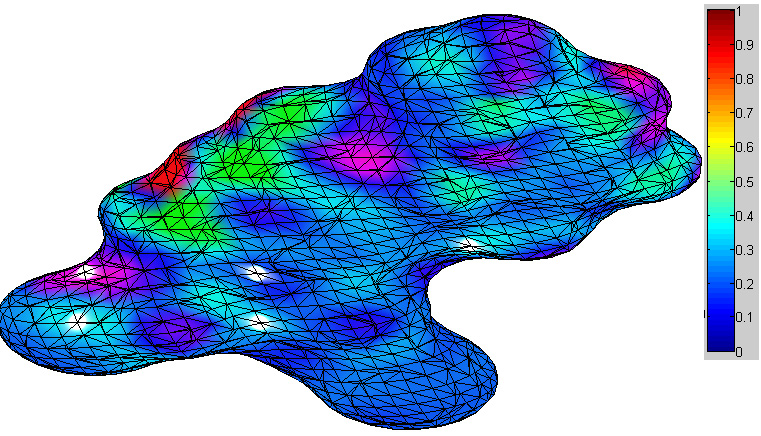
\includegraphics[scale=0.25,natwidth=761,natheight=436]{result.jpg}  
}{%
  \caption{A molecular surface with $\FRScalar$ on it and found centers (denoted by white color) 
	of blobs of radii 3.}
  \label{fig:result}
}
\capbtabbox{%
  \begin{tabular}{| l | l | l | l | l |}
    \hline
		 & $\FRScalar$ & naive & $\FRMean$ &	Adapt. \cite{GROM} \\ \hline
		glik	& 1.0 &	0.954 &	0.975 &	1.0 \\ \hline
		pirim	& 0.99 & 0.96 &	0.97 &	0.98 \\ \hline
		sesq	& 1.0 &	0.98 &	0.976 &	1.0 \\ \hline
		bzr	& 0.992 &	0.971 &	0.975 &	0.983 \\ \hline
		er\_lit & 0.98 &	0.961 &	0.956 &	0.98 \\ \hline
		cox2 & 0.991 & 0.967 & 0.985 &	0.986 \\ \hline    
  \end{tabular}
}{%
  \caption{The results: the cross-validation of models, based on feature vectors built by the blob detection methods.}%
	\label{tbl:result}
}
\end{floatrow}
\end{figure}

Riemannian blob detection with $\FRScalar$ as a blob response function is the best performing method. This shows the effectiveness of our approach. This particular method for vector-valued functions on 2D surfaces wasn't presented in the literature before. 

\section{Conclusion and Future work}
We propose the Riemannian framework for blob detection in manifold-valued images. This framework is based on the definition of blob response functions by means of image graph curvatures. Our approach gives new methods for uncovered problems and coincides with the classical blob detection for the grayscale case. The experiments results show the effectiveness of the proposed approach.
\\
The next direction for the research is a generalization of our framework to the case of sections of non-trivial fiber bundles. In particular, such generalization will cover an important case of tangent vector fields.


\begin{thebibliography}{16}
%
\bibitem{blob}
Lindeberg, T.:
Feature detection with automatic scale selection. 
International journal of computer vision, 30(2), 79--116 (1998)

\bibitem {Saucan}
Saucan, E., Wolansky, G., Appleboim, E., Zeevi, Y. Y.:
Combinatorial ricci curvature and laplacians for image processing. 
In Image and Signal Processing, CISP'09, 2nd International Congress on, 1--6 (2009)

\bibitem {Kimmel}
Sochen, N., Kimmel, R., Malladi, R.: 
A general framework for low level vision. 
IEEE transactions on image processing, 7(3), 310--318 (1998)

\bibitem {Batard}
Batard, T., Berthier, M.:
Spinor Fourier transform for image processing. 
IEEE Journal of Selected Topics in Signal Processing, 7(4), 605--613 (2013)

\bibitem {BlobCurv1}
Ferraz, L., Binefa, X.:
A sparse curvature-based detector of affine invariant blobs. 
Computer Vision and Image Understanding, 116(4), 524--537 (2012)

\bibitem {BlobCurv2}
Ferraz, L., Binefa, X.:
A scale invariant interest point detector for discriminative blob detection. 
In Iberian Conference on Pattern Recognition and Image Analysis, 233--240  (2009, June)

\bibitem {ScalarBlob3D}
Zaharescu, A., Boyer, E., Varanasi, K., Horaud, R.:
Surface feature detection and description with applications to mesh matching. 
In Computer Vision and Pattern Recognition, 2009, 373--380 (2009, June)

\bibitem {Harmonic}
Mémoli, F., Sapiro, G., Osher, S.:
Solving variational problems and partial differential equations mapping into general target manifolds. 
Journal of Computational Physics, 195(1), 263--292 (2004)

\bibitem {DTI}
Tschumperle, D., Deriche, R.:
Diffusion tensor regularization with constraints preservation. 
In Computer Vision and Pattern Recognition. CVPR 2001. Proceedings of the 2001 IEEE Computer Society Conference on (Vol. 1, pp. I-I) (2001)


\bibitem {ColorBlob}
Khanina, N. A., Semeikina, E. V., Yurin, D. V.:
Scale-space color blob and ridge detection. 
Pattern Recognition and Image Analysis, 22(1), 221--227 (2012)

\bibitem {GROM}
Smirnov, P., Semenov, P., Lyakh, M., Chun, A., Gusev, D., Redkin, A., Srinivasan, S.:
GRoM—Generalized robust multichannel feature detector. 
In Signal and Image Processing Applications, 2011 IEEE International Conference on, 585--590 (2011, November)

\bibitem {DiffGeom}
Spivak, M.: 
Comprehensive introduction to differential geometry.
Vol. IV A (1981)

\bibitem {qsar}
Baskin, I., Varnek, I.:
Fragment Descriptors in SAR/QSAR/QSPR Studies, Molecular Similarity Analysis and in Virtual Screening.
Chemoinformatic Approaches to Virtual Screening, 1--43 (2008)

\bibitem {molecular}
Connolly, M. L.:
Analytical molecular surface calculation. 
Journal of Applied Crystallography, 16(5), 548--558 (1983)

\bibitem {bag}
Csurka, G., Dance, C., Fan, L., Willamowski, J., Bray, C.: 
Visual categorization with bags of keypoints. 
In Workshop on statistical learning in computer vision, ECCV, Vol. 1, No. 1-22, 1--2 (2004, May). 

\bibitem {cross}
Kohavi, R.:
A study of cross-validation and bootstrap for accuracy estimation and model selection. 
In Ijcai, Vol. 14, No. 2, 1137--1145 (1995, August)

\bibitem {SVM}
Weston, J., Mukherjee, S., Chapelle, O., Pontil, M., Poggio, T., Vapnik, V.:
Feature selection for SVMs. 
In Proceedings of the 13th International Conference on Neural Information Processing Systems, 647--653 (2000, January)

\bibitem {kernel}
J. J. Sutherland, L. A. O’Brien, and D. F. Weaver.:
Spline-fitting with a genetic algorithm : a method for developing classification structure-activity relationships.
J. Chem. Inf. Comput. Sci., 43:1906–1915 (2003)

\end{thebibliography}

\end{document}